\chapter{Résolution de problèmes \textsf{\#P}-complet avec VQCount}
\label{cha:resolution-de-problemes-avec-vqcount}
%-----------------------------------------------------------------------------%

Dans le chapitre précédent, un cadre théorique s'appuyant sur l'algorithme de JVV a été construit pour la résolution de problèmes de comptage à l'aide d'algorithmes variationnels quantiques. L'algorithme résultant, VQCount, obtient un compte approximatif à une erreur multiplicative près en échantillonnant un nombre polynomial de solutions à un circuit quantique optimisé GM-QAOA. Toutefois, plusieurs conditions potentiellement dispensables ou difficilement applicables ont été imposées. Ce chapitre change l'optique précédente en évaluant l'algorithme VQCount uniquement en tant que méthode heuristique, c'est-à-dire en caractérisant l'algorithme sans se soucier des garanties. La résolution de deux problèmes \textsf{\#P}-complet, \#NAE3SAT et \#1in3SAT, est alors étudiée à l'aide de simulations de réseaux de tenseurs.

La section~\ref{sec:parametres-de-etude} définit les paramètres des simulations numériques effectuées et la section~\ref{sec:methode} explique la méthode utilisée pour caractériser l'algorithme VQCount. La performance de VQCount est examinée aux sections~\ref{sec:biais-echantillonnage} et~\ref{sec:comportement-echelle}, où l'impact du biais d'échantillonnage des circuits QAOA et le comportement d'échelle sont respectivement présentés.

Le projet de ce mémoire a mené au développement d'un module python, nommé VQCount, disponible sur GitHub (\url{https://github.com/QuICoPhy-Lab/VQCount}). Ce module a été utilisé pour les simulations numériques de ce chapitre. 

%-----------------------------------------------------------------------------%

\section{Paramètres de l'étude}
\label{sec:parametres-de-etude}

Certaines précédentes considérations sont relâchées ou modifiées. D'abord, 
l'algorithme GM-QAOA n'est plus considéré dans sa forme limite de Grover. Plutôt qu'utiliser les paramètres fixes $\gamma_{i}=\beta_{i}=\pi$ pour $i=1,\dots,p$ dans le circuit GM-QAOA, les paramètres sont optimisés. De plus, les problèmes étudiés sont transformés à des hamiltoniens de problème contenant une tour d'états excités plutôt que de l'oracle à deux niveaux construit précédemment. Comme l'impact de la non-uniformité de la distribution d'état produite est étudié, l'algorithme VQCount est aussi employé avec l'algorithme quantique d'optimisation approximative. Cette section utilise donc QAOA pour référer à ce dernier. Finalement, la procédure d'auto-réduction de la section~\ref{sec:procedure-auto-reduction} est utilisée en renonçant à la réoptimisation des paramètres à chaque étape.

Pour les simulations numériques effectuées, les solutions sont échantillonnées sans remplacement. Ce choix s'écarte du protocole de l'algorithme de JVV, mais il accroît l'efficacité de la méthode lorsqu'un problème présente peu de solutions ou lorsque la distribution préparée par le circuit est fortement non-uniforme.

L'algorithme VQCount est appliqué aux problèmes \#NAE3SAT positif et \#1-in-3SAT positif présentés à la section~\ref{sec:satisfaisabilite-booleenne}. Le problème \#NAE3SAT est difficile près du seuil de satisfaisabilité critique situé au rapport de clauses sur variables $\alpha_{c} \approx 2.1$. Pour étudier l'effet de la complexité des formules aléatoires sur la performance de VQCount, des instances sont générées à $\alpha = 1$ et $\alpha = 2$. Celles-ci sont générées à partir de graphes connectés bipartis, imposant une restriction supplémentaire. Similairement, les instances du problème positif \#1-in-3SAT sont à leur seuil de difficulté le plus élevé près de $\alpha_{c} \approx 2/3$. Pour étudier ce problème dans le régime difficile, les instances sont générées à partir de graphes aléatoires cubiques, en plaçant une clause sur tous les sommets et une variable sur toutes les arêtes. Cette méthode permet d'échantillonner uniformément les instances difficiles, éliminant le biais dû à une sélection aléatoire~\cite{vigerEfficientSimpleGeneration2005}. Ce type de problème appartient à la catégorie des problèmes bloqués, étant vraisemblablement les plus difficiles des problèmes \textsf{\#P}. Par la suite, les instances générées sont converties en un modèle d'Ising à l'aide de la transformation décrite à la section~\ref{subsec:encodage-probleme}.

La simulation de circuits quantiques est un problème complexe en raison de la quantité de mémoire nécessaire pour représenter l'espace de Hilbert. La méthode la plus utilisée, la simulation à vecteur d'état, ne peut atteindre plus d'une vingtaine de qubits pour cette raison. Les réseaux de tenseurs sont un outil alternatif puissant, particulièrement pour l'étude de circuits quantiques peu profonds. L'annexe~\ref{ann:simulation-circuits-quantiques-avec-reseaux-de-tenseurs} introduit les réseaux de tenseurs et les méthodes particulières utilisées pour la simulation de l'algorithme VQCount. La librairie « quimb »~\cite{grayQuimbPythonPackage2018} est utilisée pour modéliser l'optimisation et l'échantillonnage des circuits quantiques QAOA et GM-QAOA. Les paramètres de ces circuits sont optimisés avec la programmation séquentielle des moindres carrés, telle qu'implémentée par la librairie « SciPy »~\cite{virtanenSciPy10Fundamental2020}. Pour évaluer la validité des résultats obtenus, « Ganak »~\cite{sharmaGANAKScalableProbabilistic2019}, un compteur de modèles exact fondé sur une approche probabiliste, est utilisé pour déterminer le nombre exact de solutions. Le solveur SAT « Glucose4 »~\cite{eenExtensibleSATsolver2004,audemardPredictingLearntClauses2009}, implémenté dans l'ensemble d'outils « PySAT »~\cite{ignatievPySATPythonToolkit2018}, est employé pour énumérer toutes les solutions possibles.

Pour le problème \#NAE3SAT, 20 instances aléatoires sont générées par taille d'instance, allant de 6 à 20 variables, pour les deux densités de clause $\alpha=1$ et $\alpha = 2$. Similairement, problème \#1-in-3SAT, 20 instances aléatoires sont générées pour une taille de variable allant de 9 à 27 variables par saut de 3 variables, pour une densité de clause $\alpha = 2/3$. 

%-----------------------------------------------------------------------------%

\section{Méthode}
\label{sec:methode}
\begin{figure}[ht!]
    \centering
    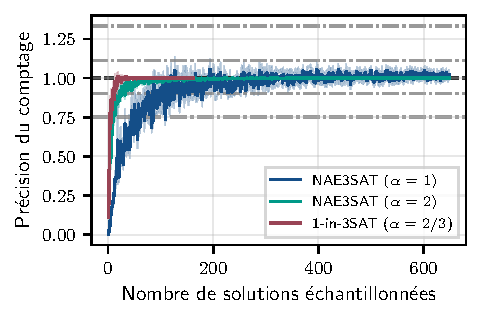
\includegraphics[width=0.6\textwidth]{figures/count-accuracy.pdf}
    \caption[Précision du comptage pour des problèmes \textsf{\#P}-difficile]{Précision du comptage obtenue en augmentant le nombre de solutions échantillonnées à chaque étape de la procédure d'auto-réduction avec des circuits QAOA de profondeur $p=3$ pour les instances NAE3SAT et 1-in-3SAT avec $n=18$ variables. Les lignes solides représentent la moyenne et les régions ombragées montrent l'erreur standard de la moyenne. La ligne noire en pointillés représente la précision exacte du comptage, tandis que les lignes grises en tirets et pointillés correspondent à une erreur multiplicative de $\varepsilon = 1/3$ et $\varepsilon = 1/9$.}
    \label{fig:count-accuracy.pdf}
\end{figure}

Afin de déterminer le nombre d'échantillons nécessaires pour atteindre un compte approximatif avec une tolérance $\varepsilon$ et une confiance $\delta$, le nombre d'échantillons utilisé par l'algorithme VQCount devrait être augmenté jusqu'à ce que le nombre de solutions trouvé soit à une erreur multiplicative $\varepsilon$ du nombre de solutions exact avec une probabilité supérieure à $\delta$. La simulation de l'algorithme étant coûteuse, une méthode plus simple et moins rigoureuse est utilisée ici. L'algorithme VQCount est exécuté en augmentant le nombre de solutions échantillonnées du circuit quantique optimisé QAOA jusqu'à ce que le nombre de solutions soit à l'intérieur des bornes d'erreur $\varepsilon$. La figure~\ref{fig:count-accuracy.pdf} montre la précision du comptage, c'est-à-dire le rapport du nombre de solutions approximatif sur le nombre de solutions exact, pour différentes erreurs multiplicatives $\varepsilon$. Notons que, pour réduire les incertitudes, une procédure de lissage est utilisée. L'algorithme de JVV semble sous-estimer le nombre de solutions, comme vu avec la courbe de \#NAE3SAT avec $\alpha = 1$. Ce comportement s'explique par le manque d'échantillons indiscernables dans la distribution de probabilité des solutions échantillonnées, entraînant une inexactitude des probabilités dans l'arbre d'auto-réductibilité. 

%-----------------------------------------------------------------------------%

\section{Biais d'échantillonnage}
\label{sec:biais-echantillonnage}

\begin{figure}[ht!]
    \centering
    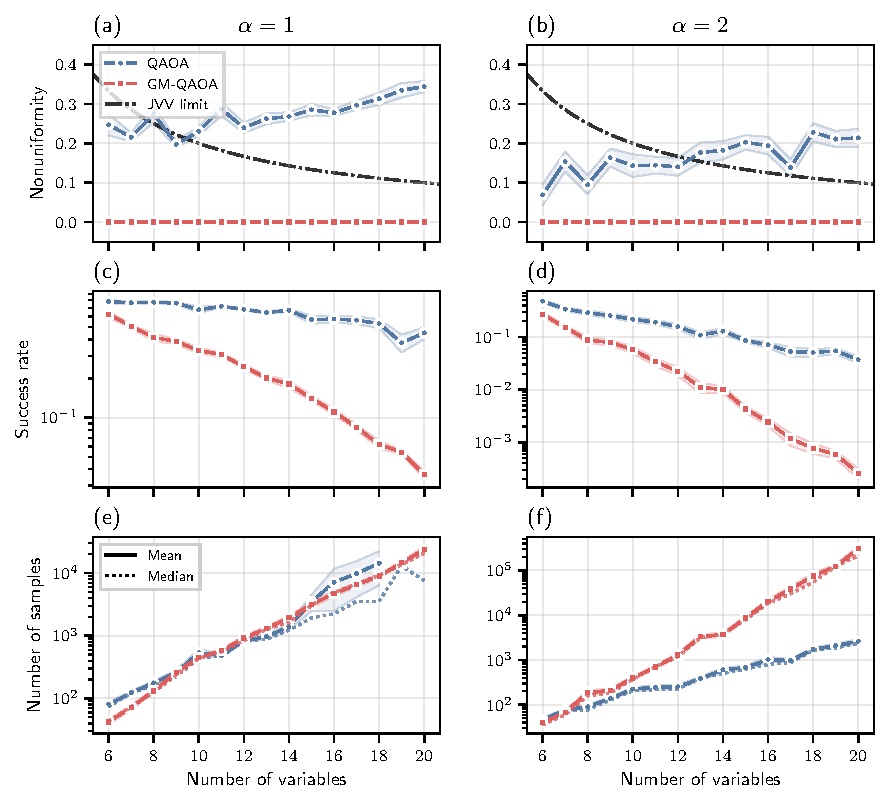
\includegraphics[width=1\textwidth]{figures/nae3sat-nonuniformity.pdf}
    \caption[Biais d'échantillonnage pour \#NAE3SAT]{Performance de VQCount avec des circuits QAOA de profondeur $p=3$ (cercles bleus) et GM-QAOA (carrés rouges) pour les instances NAE3SAT à $\alpha=1$ (panneaux de gauche) et $\alpha=2$ (panneaux de droite). Les lignes solides et pointillées représentent respectivement la moyenne et la médiane. Les régions ombragées montrent l'erreur standard de la moyenne. (a,b) Non-uniformité maximale tout au long de la procédure d'auto-réduction. L'algorithme JVV nécessite que la non-uniformité soit au plus $O(n^{-1})$ pour $n$ variables, comme illustré (lignes noires en tirets et pointillés) avec la fonction $f(n) = O(1/n)$. (c,d) Taux de succès minimal tout au long de la procédure d'auto-réduction. (e,f) Nombre d'échantillons nécessaires pour obtenir un comptage approximatif avec une tolérance d'erreur $\varepsilon = 1/3$. Un ajustement exponentiel extrapolé à partir des cinq derniers points de la médiane donne $O(1.45^n)$ (QAOA) et $O(1.44^n)$ (GM-QAOA) pour (e), et $O(1.34^n)$ (QAOA) et $O(1.88^n)$ (GM-QAOA) pour (f).}
    \label{fig:nae3sat-number-of-samples}
\end{figure}

Comme vu à la section~\ref{sec:echantillonnage-et-biais}, l'état préparé par un circuit GM-QAOA permet un échantillonnage uniforme de solutions tel que nécessaire pour l'algorithme de JVV, alors que la probabilité de certaines solutions est exponentiellement réduite avec l'approche QAOA. Sachant que les problèmes étudiés possèdent en moyenne un nombre exponentiel de solutions alors que seul un nombre polynomial d'échantillons est nécessaire, il est possible que la distribution préparée par QAOA soit suffisante pour obtenir un compte approximatif convenable. La figure~\ref{fig:nae3sat-number-of-samples} résume les résultats obtenus pour le problème \#NAE3SAT avec un circuit de profondeur $p=3$. Les figures~\ref{fig:nae3sat-number-of-samples}(a) et~\ref{fig:nae3sat-number-of-samples}(b) confirment que GM-QAOA échantillonne les solutions parfaitement uniformément. Au contraire, la distribution des solutions préparées par QAOA est de plus en plus non-uniforme avec la taille de l'instance. 

Les figures~\ref{fig:nae3sat-number-of-samples}(c) et~\ref{fig:nae3sat-number-of-samples}(d) montrent que, pour une profondeur de circuit fixe, le taux de succès de QAOA et GM-QAOA diminue grossièrement de façon exponentielle avec le nombre de variables, bien que la diminution soit plus importante pour GM-QAOA. Les taux de succès sont plus faibles et se détériorent plus rapidement pour les instances avec $\alpha = 2$ qu'avec $\alpha=1$, reflétant la différence de complexité de celles-ci selon leur proximité avec le seuil de satisfaisabilité. 

Le nombre total d'échantillons requis pour que l'algorithme VQCount retourne un compte approximatif à une erreur multiplicative $\varepsilon = 1/3$ est présenté à la figure~\ref{fig:nae3sat-number-of-samples}(e) et~\ref{fig:nae3sat-number-of-samples}(f). Le nombre d'échantillons augmente exponentiellement avec la taille des instances en raison de la post-sélection des solutions à la fois pour QAOA et GM-QAOA comme générateurs de solutions. Bien que le taux de succès de GM-QAOA soit exponentiellement inférieur à QAOA, VQCount nécessite environ le même nombre d'échantillons avec QAOA ou GM-QAOA pour $\alpha=1$. Au contraire, VQCount avec QAOA nécessite un nombre exponentiellement plus petit que celui de GM-QAOA, malgré la non-uniformité de la distribution des probabilités de QAOA. Cela suggère que QAOA est potentiellement un générateur plus efficace pour VQCount dans le cas où les solutions soient rares et dispersées. Le nombre d'échantillons post-sélectionnés requis pour que VQCount produise un estimé à un facteur multiplicatif $\varepsilon$ près du compte exact, présenté à la figure~\ref{fig:nae3sat-scaling}, semble polynomial selon le nombre de variables $n$ et l'inverse de la tolérance $1/\varepsilon$ comme attendu.

\begin{figure}[ht!]
    \centering
    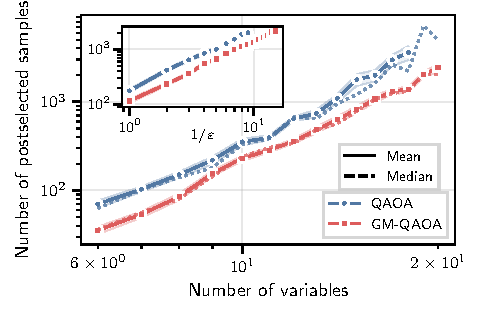
\includegraphics[width=0.6\textwidth]{figures/nae3sat-scaling.pdf}
    \caption[Comportement d'échelle du nombre d'échantillons post-sélectionnés pour \#NAE3SAT]{Nombre d'échantillons post-sélectionnés nécessaires pour obtenir un comptage approximatif avec une tolérance d'erreur $\varepsilon=1/3$ avec des circuits QAOA de profondeur $p=3$ (cercles bleus) et GM-QAOA (carrés rouges) pour les instances NAE3SAT à $\alpha=1$. Les lignes solides et pointillées représentent respectivement la moyenne et la médiane. Les régions ombragées montrent l'erreur standard de la moyenne. Un ajustement polynomial de la médiane donne $O(n^{5.12})$ (QAOA) et $O(n^{3.42})$ (GM-QAOA). Le panneau inséré montre le comportement de l'échelle en fonction de l'inverse de la tolérance d'erreur $\varepsilon$ pour $n=12$ variables. Un ajustement polynomial de la moyenne donne $O(\varepsilon^{-1.13})$ (QAOA) et $O(\varepsilon^{-1.07})$ (GM-QAOA).}
    \label{fig:nae3sat-scaling}
\end{figure}

Sachant qu'un problème de plus petite taille est échantillonné à chaque étape de l'algorithme de JVV, il est raisonnable, du moins en théorie, de s'attendre à ce que le taux de succès de l'algorithme augmente. Cependant, dans cette étude, les paramètres du circuit quantique sont optimisés une seule fois et maintenus à des valeurs fixes au cours de la procédure d'auto-réduction, comme la réoptimisation est coûteuse à simuler classiquement. Est-ce que ce choix a un impact important sur la performance de l'algorithme VQCount? Comme montré à la section~\ref{sec:procedure-auto-reduction}, le taux de succès ne diminue pas avec le nombre d'étapes dans la limite de Grover. La figure~\ref{fig:nae3sat-jvv-steps} vérifie alors si cette hypothèse tient même en s'éloignant de cette limite. Les taux de succès demeurent effectivement non décroissants pour GM-QAOA. En revanche, la non-uniformité de QAOA augmente initialement avant de diminuer, comme vue dans la figure~\ref{fig:nae3sat-jvv-steps}(a,b), avec une augmentation plus prononcée pour $\alpha = 1$. Ce comportement corrèle avec une diminution du taux de succès dans les premières étapes de l'auto-réduction. Le taux de succès de QAOA est toutefois toujours plus grand que celui de GM-QAOA. 

\begin{figure}[ht!]
    \centering
    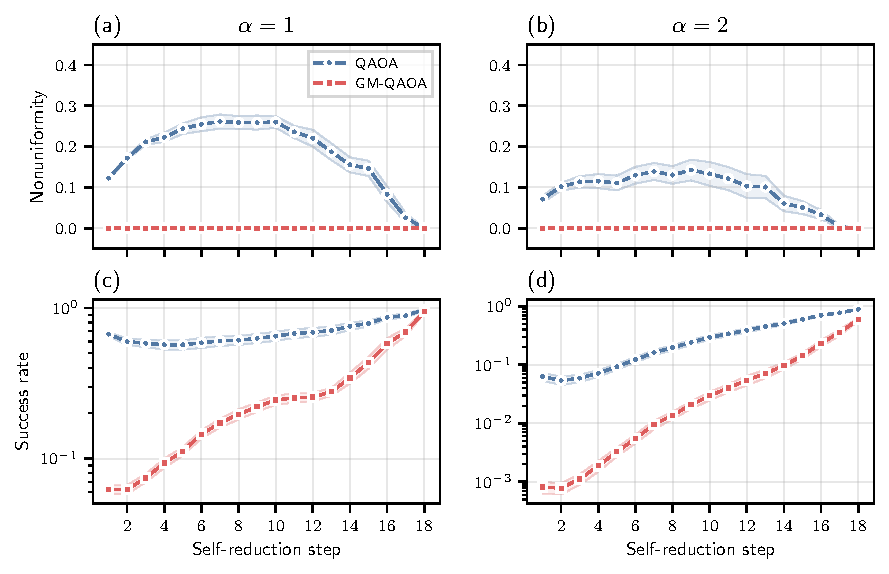
\includegraphics[width=1\textwidth]{figures/nae3sat-self-reduction-step.pdf}
    \caption[Impact de la procédure d'auto-réduction sur la non-uniformité pour \#NAE3SAT]{Impact de la fixation des qubits tout au long de la procédure d'auto-réduction sur l'échantillonnage avec des circuits QAOA de profondeur $p=3$ (cercles bleus) et GM-QAOA (carrés rouges) pour les instances NAE3SAT de $n=18$ variables à $\alpha=1$ (panneaux de gauche) et $\alpha=2$ (panneaux de droite). Les lignes solides représentent la moyenne et les régions ombragées montrent l'erreur standard de la moyenne. (a,b) Non-uniformité en fonction du nombre d'étapes dans procédure d'auto-réduction. (c,d) Taux de succès en fonction du nombre d'étapes dans la procédure d'auto-réduction.}
    \label{fig:nae3sat-jvv-steps}
\end{figure}

Pour l'instant, la performance de VQCount a été étudiée pour des circuits de profondeur fixe. La figure~\ref{fig:nae3sat-depth} montre que, lorsque la profondeur du circuit augmente, la non-uniformité diminue et la probabilité d'obtenir une solution augmente, menant à un moindre nombre d'échantillons nécessaires pour atteindre un compte approximatif avec une erreur multiplicative donnée. QAOA semble s'améliorer plus rapidement selon la profondeur du circuit que GM-QAOA. D'autre part, la non-uniformité de QAOA augmente et atteint un plateau avec la profondeur du circuit.

\begin{figure}[ht!]
    \centering
    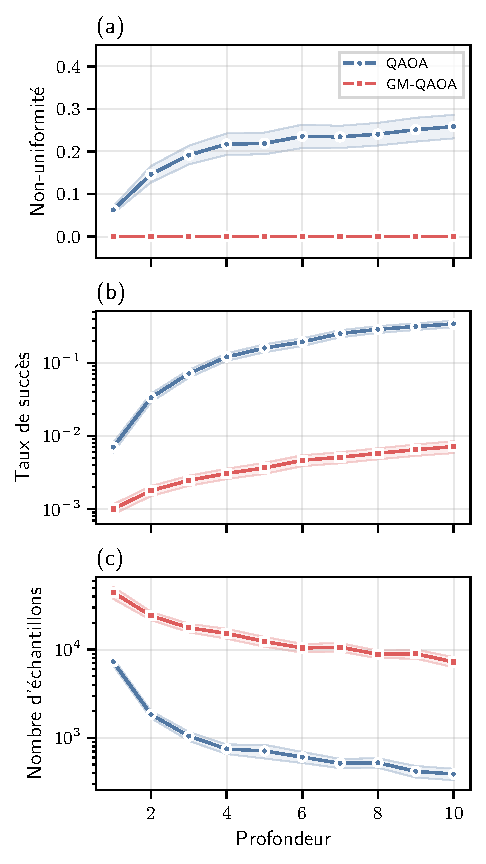
\includegraphics[width=0.5\textwidth]{figures/nae3sat-depth.pdf}
    \caption[Impact de la profondeur du circuit pour \#NAE3SAT]{Performance de VQCount en fonction de la profondeur avec des circuits QAOA (cercles bleus) et GM-QAOA (carrés rouges) pour les instances NAE3SAT de $n=16$ variables à $\alpha=2$. Les lignes solides représentent la moyenne et les régions ombragées montrent l'erreur standard de la moyenne. (a) Non-uniformité maximale tout au long de la procédure d'auto-réduction. (b) Taux de succès minimal tout au long de la procédure d'auto-réduction. (c) Nombre d'échantillons nécessaires pour obtenir un comptage approximatif avec une tolérance d'erreur $\varepsilon = 1/3$.}
    \label{fig:nae3sat-depth}
\end{figure}

Les résultats précédents suggèrent que, pour une faible profondeur de circuit, le circuit QAOA constitue un générateur de solutions plus efficace que le circuit GM-QAOA. Ce dernier dépend de plus d'une porte contrôlée à $n$ qubits, difficile à simuler classiquement et peu compatible avec les ordinateurs quantiques bruités à court terme. Ainsi, la section suivante se concentre sur l'évaluation des performances de VQCount en utilisant le générateur de solutions QAOA.

%-----------------------------------------------------------------------------%

\section{Comportement d'échelle}
\label{sec:comportement-echelle}

\begin{figure}[ht!]
    \centering
    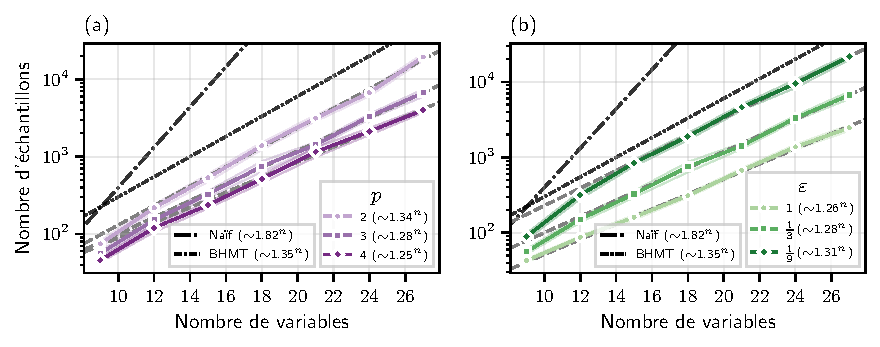
\includegraphics[width=1\textwidth]{figures/1in3sat-number-of-samples.pdf}
    \caption[Comportement d'échelle du nombre d'échantillons pour \#1-in-3SAT]{Comportement de mise à l'échelle de VQCount avec des circuits QAOA pour les instances 1-in-3SAT à $\alpha=2/3$. Le nombre d'échantillons nécessaires pour obtenir un comptage approximatif en utilisant l'échantillonnage par rejet naïf et l'algorithme de comptage quantique de Brassard, Høyer, Mosca et Tapp (BHMT) est indiqué respectivement par une ligne noire en tirets et pointillés et une ligne noire en tirets densément pointillés, suivant les fonctions $f(n) = O(1.82^{n})$ et $f(n) = O(1.35^{n})$ pour $n$ variables. Les lignes solides représentent la moyenne, et les régions ombragées montrent l'erreur standard de la moyenne. Les lignes en pointillés indiquent l'ajustement exponentiel extrapolé à partir des quatre derniers points, comme indiqué dans la légende. (a) Nombre d'échantillons nécessaires pour que le comptage approximatif soit dans la tolérance d'erreur $\varepsilon = 1/3$ pour les profondeurs $p$. (b) Nombre d'échantillons nécessaires pour que le comptage approximatif soit dans la tolérance d'erreur $\varepsilon$ pour une profondeur $p=3$.}
    \label{fig:1in3sat-number-of-samples}
\end{figure}

Ayant conclu que QAOA semble être un meilleur générateur de solutions pour une faible profondeur de circuit, la performance de VQCount avec QAOA est caractérisée de manière approfondie pour le problème \#1-in-3SAT. La figure~\ref{fig:1in3sat-number-of-samples} résume le comportement de mise à l'échelle de VQCount avec un circuit QAOA de faible profondeur. Naïvement, le nombre de solutions peut être trouvé en déterminant la probabilité qu'une chaîne de bit aléatoire échantillonnée de l'ensemble des chaînes de bits possible soit une solution. Comme vu à la figure~\ref{fig:1in3sat-number-of-samples}(a), VQCount possède une loi d'échelle exponentiellement meilleure qu'avec l'échantillonnage par rejet naïf et sa performance s'améliore avec la taille du circuit. De plus, sa performance se compare à l'algorithme quantique de comptage approximatif de Brassard, H\o yer, Mosca et Tapp~\cite{brassardQuantumAmplitudeAmplification2002}, qui possède un comportement d'échelle $O(\sqrt{N/M})$ pour une taille d'espace de solutions $M$ et une taille de l'espace de recherche total $N$. Aux profondeurs de circuits accessibles avec des ressources computationnelles raisonnables, l'efficacité asymptotique de VQCount est inférieure à celle des algorithmes classiques de pointe pour ce problème~\cite{kourtisFastCountingTensor2019}. Cependant, les résultats suggèrent que ce n'est possiblement pas le cas pour des profondeurs de circuit finies plus grandes. La précision de VQCount peut être améliorée en augmentant le nombre d'échantillons, comme montré à la figure \ref{fig:1in3sat-number-of-samples}(b). Finalement, la figure~\ref{fig:1in3sat-scaling} montre le nombre d'échantillons post-sélectionnés nécessaire pour produire un compte à un facteur multiplicatif $\varepsilon$ près du nombre de solutions exact en fonction du nombre de variables et de l'inverse de la tolérance. Ces résultats suggèrent un comportement d'échelle superpolynomial, mais sous-exponentiel du nombre d'échantillons post-sélectionnés nécessaires. 

\begin{figure}[H]
    \centering
    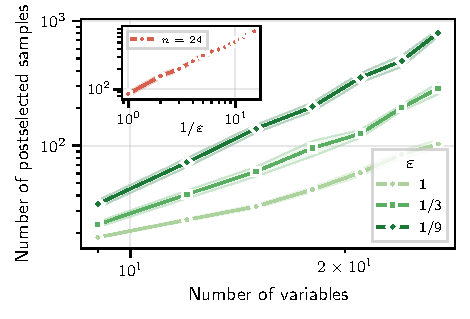
\includegraphics[width=0.6\textwidth]{figures/1in3sat-scaling.pdf}
    \caption[Comportement d'échelle du nombre d'échantillons post-sélectionnés pour \#1-in-3SAT]{Nombre d'échantillons post-sélectionnés nécessaires pour obtenir un comptage approximatif avec une tolérance d'erreur $\varepsilon$ avec des circuits QAOA de profondeur $p=3$ pour les instances 1-in-3SAT à $\alpha=2/3$. Le panneau inséré montre le comportement de mise à l'échelle en fonction de l'inverse de la tolérance d'erreur $\varepsilon$ pour $n=24$ variables, pour lequel un ajustement polynomial donne $O(\varepsilon^{-0.79})$. Les lignes solides représentent la moyenne, et les régions ombragées montrent l'erreur standard de la moyenne.}
    \label{fig:1in3sat-scaling}
\end{figure}

L'algorithme VQCount permet d'estimer un nombre exponentiel de solutions en utilisant seulement un nombre polynomial d'échantillons. Toutefois, dans les simulations numériques, certaines instances de problème peuvent comporter un petit nombre de solutions. Il est donc essentiel de vérifier que VQCount requiert, en pratique, moins d'échantillons que le nombre total de solutions, afin d'éviter une simple énumération exhaustive. La figure~\ref{fig:sampling-efficiency} illustre l'efficacité d'échantillonnage de VQCount, définie comme le rapport entre le nombre exact de solutions et le nombre de solutions distinctes utilisées par l'algorithme, pour les deux problèmes étudiés dans ce travail. L'efficacité d'échantillonnage est positivement corrélée à la densité des solutions. Néanmoins, VQCount utilise systématiquement moins d'échantillons que le nombre total de solutions.

\begin{figure}[ht!]
    \centering
    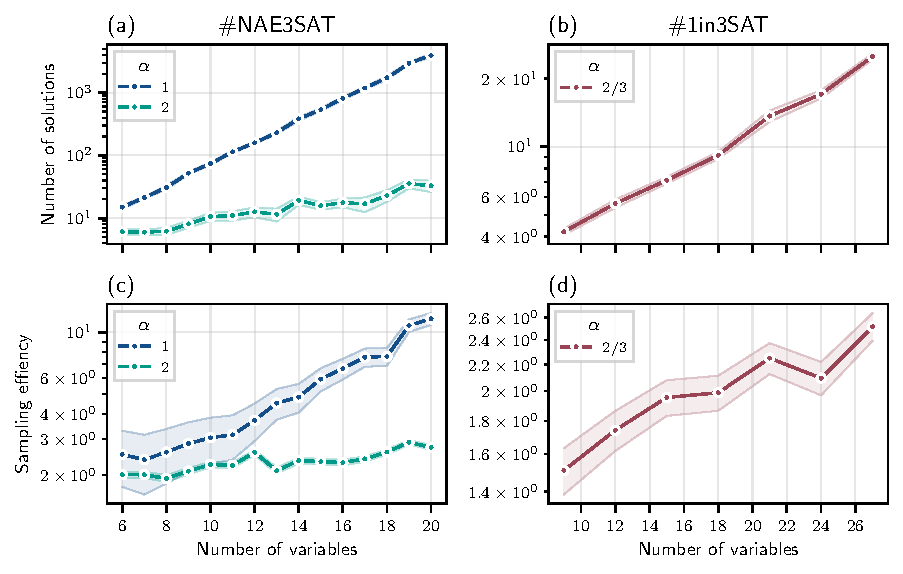
\includegraphics[width=1\textwidth]{figures/sampling-efficiency.pdf}
    \caption[Efficacité de l'échantillonnage pour des problèmes \#P-difficile]{Nombre de solutions (a) et efficacité d'échantillonnage (b) pour atteindre une tolérance d'erreur $\varepsilon = 1$ avec des circuits QAOA de profondeur $p=3$ pour les instances NAE3SAT (panneaux de gauche) et 1-in-3SAT (panneaux de droite). Les lignes solides représentent la moyenne, et les régions ombragées montrent l'erreur standard de la moyenne.}
    \label{fig:sampling-efficiency}
\end{figure}

%-----------------------------------------------------------------------------%

